% Compile twice with pdfLaTeX. Figures and bibliography are included.
% Source materials: AI教練提案解析.pdf, AI_Fitness_Coach.png, A2Z outline example.pdf
\documentclass[conference]{IEEEtran}
\usepackage{amsmath,booktabs,tabularx,array,tikz,algorithmic}
\usetikzlibrary{arrows.meta,positioning}
\usepackage[hidelinks]{hyperref}
\newcolumntype{Y}{>{\raggedright\arraybackslash}X}
\tikzset{box/.style={draw,rounded corners=2pt,align=center,inner sep=4pt,font=\footnotesize},link/.style={-{Stealth[length=4pt]},thin}}
\begin{document}
\title{AI Fitness Coach: A Conversational Running Coach for Quota-Limited Cloud Deployment}
% Replace the draft label with verified author names and affiliations.
\author{\IEEEauthorblockN{Project proposal}}
\maketitle
\begin{abstract}
% A -- Attention getter
In Strava's 2025 survey, 46\% of respondents said they would use AI for sports coaching. One practical question is whether a runner can finish a route before rain is forecast.
% B -- Challenge
On a 5~km loop, a one-minute-per-kilometre pace error shifts the finish by five minutes. A coach that guesses the pace or reuses a forecast for an earlier departure can reverse the answer even when its arithmetic is correct.
% C -- Cure
AI Fitness Coach asks for the missing input and combines the confirmed pace, route length and local forecast in one reply.
% D -- Development
A browser connects a single agent to running and nutrition tools. A scope check and a usage budget govern calls, and the runner can read the reply or hear it through a lip-synchronized avatar.
% E -- Experiments
The project used a scripted demonstration on a free cloud tier. We specify a follow-up comparison with a form and a locally deployed agent to measure correct task completion, token use and response time.
% F -- Findings
For a 32-minute window our calculation gives a break-even pace of 6:24 min/km over 5~km. The project reports an end-to-end run spanning conversation, weather and route lookup, manual exercise logging, food analysis, menu retrieval and avatar playback. The demonstration establishes that these functions ran together. Per-attempt measurements are still needed to determine whether page queries meet the proposed 2~s target and spoken replies the 12~s target at the 95th percentile.
\end{abstract}
\begin{IEEEkeywords}
conversational agents, running, tool calling, voice interaction, latency
\end{IEEEkeywords}
\section{Introduction}
Strava's 2025 report drew on a survey of more than 30,000 people, including users and non-users of its platform. Among respondents, 46\% expressed willingness to use AI for sports coaching~\cite{strava}. This measures stated interest. Whether a runner can act on a particular reply depends on how the coach handles details the runner leaves out.

Consider a runner asking if their usual loop fits before the rain. A route planner can supply the distance and a weather service can supply the forecast. The runner still has to combine them with a departure time and a realistic pace. Table~\ref{tab:margin} shows why the coach should ask for pace. At 6:00 min/km the runner has two minutes to spare. At 6:30 min/km the same route takes half a minute too long. Asking again for an already confirmed distance, by comparison, would cost a turn without resolving the decision.

\begin{table}[!b]
\caption{Illustrative 5~km loop starting at 17:00 with rain forecast at 17:32. Positive margin means finishing before forecast onset.}
\label{tab:margin}\centering\small
\begin{tabular}{@{}lrrr@{}}\toprule
Pace (min/km) & Run (min:s) & Finish & Margin (min:s)\\\midrule
6:00 & 30:00 & 17:30:00 & $+$2:00\\
6:30 & 32:30 & 17:32:30 & $-$0:30\\
7:00 & 35:00 & 17:35:00 & $-$3:00\\\bottomrule
\end{tabular}
\end{table}
These examples assume constant pace and no stops. If the weather service gives an onset window, the reply should retain it. An uncertainty of several minutes can erase the two-minute margin in the first row.
The coach supports run interpretation, pace calculation, weather and route lookup, and meal queries~\cite{proposal}. Sections~II and III give the evidence and system design. Section~IV specifies the comparison and Section~V describes the remaining work.

\section{Related Work}
ReAct lets an agent revise its next action after observing a tool result~\cite{react}. This matters when a runner changes the departure time after a forecast lookup. PH-LLM used expert assessments of replies about wearable data~\cite{phllm}, a precedent for checking content separately from fluency.

El Helou \emph{et al.} analyzed 1,791,972 finish records from 60 marathons in six cities over 2001--2010~\cite{heat}. Mean running speed fell above the temperature associated with peak speed, which varied by performance level. The study supports checking local conditions. Applying a numerical pace adjustment to a recreational 5~km run would require data for that distance and population. Table~\ref{tab:papers} connects the evidence to design decisions. The open question is whether the coach can give a correct, timely answer when a turn needs both arithmetic and external data.

\begin{table*}[t]
\caption{Article Summary Table. Six primary studies and the limits of applying their results to a running coach.}
\label{tab:papers}\centering\small
\renewcommand{\arraystretch}{1.10}
\begin{tabularx}{\textwidth}{@{}p{2.10cm}YYYY@{}}\toprule
Article / year & Research question and method & Domain and data & Published finding & Relevance and limit\\\midrule
Yao et al.~\cite{react}, 2023 & Does interleaving reasoning with tool actions improve task success? Compare ReAct with action-only prompting. & Interactive decision making in WebShop, a simulated shopping environment. & Success was 40.0\% with ReAct and 30.1\% with action-only prompting (Table~4 of the paper). & Keep tool observations available for later turns. A shopping success rate gives no estimate of running-task accuracy.\\\addlinespace
Yao et al.~\cite{tau}, 2024 & Can an agent consistently complete a task over repeated conversations? Compare final database states with goal states. & Simulated users, domain policies and tool calls for airline and retail service. & In retail, the reported probability of success on all eight repeated trials was below 25\% for GPT-4o. & Judge a saved run by its final stored fields. Repetition tests reliability beyond one successful demonstration.\\\addlinespace
Khasentino et al.~\cite{phllm}, 2025 & Can a fine-tuned model interpret wearable data? Experts rated generated coaching responses. & 857 sleep and fitness cases, including 100 held out for evaluation. & Experts rated the model similarly to human experts on the fitness tasks. & Score reply content separately from speed. The study evaluated fitness advice from wearable summaries.\\\addlinespace
El Helou et al.~\cite{heat}, 2012 & Which weather variables track marathon performance? Link race-day observations with finish records. & 1,791,972 finishes across 60 marathons in six cities, 2001--2010. & Above the temperature associated with peak mean speed, runners slowed. The peak varied by performance level. & Include weather context. The population does not establish a temperature correction for an individual 5~km outing.\\\addlinespace
Gilgen-Ammann et al.~\cite{gnss}, 2020 & How closely do sport watches record known distances? Compare devices against measured routes. & Eight watches, three environments and 36 planned trials per watch. One participant walked, ran and cycled. & Device-level mean absolute percentage errors ranged from 3.2\% to 6.1\% across environments. & Keep the distance source with a saved pace. These device averages do not bound a future phone's error.\\\addlinespace
Thames et al.~\cite{nutri}, 2021 & Can images support nutrient estimation? Evaluate predictions against labels derived from ingredient weights. & Nutrition5k contains roughly 5,000 cafeteria dishes with images, depth and ingredient measurements. & Across dishes, energy averaged 255~kcal (SD 220) and mass averaged 215~g (SD 161). & Preserve the portion basis of a food entry. Cafeteria dish measurements do not establish accuracy on a runner's own photo.\\\bottomrule
\end{tabularx}
\end{table*}


\subsection{What counts as a successful answer?}
The outcome in each study determines what can be carried into this design. On WebShop, the gap between ReAct and action-only prompting was 9.9 percentage points~\cite{react}. Both systems could act. The comparison therefore motivates testing how an agent uses a returned observation once it has one. In our case, a trace can show a successful weather lookup even if the final sentence quotes yesterday's forecast. A test should inspect the time and place used in the reply as well as the invocation of the tool.

For a request that writes a record, the relevant evidence is the record after the conversation. In $\tau$-bench, Yao \emph{et al.} compared the database at the end of a task with the intended state~\cite{tau}. A running analogue is a user who corrects a distance from 5 to 4~km after logging a 30-minute run. The expected record has one run, 4~km and a pace of 7:30 min/km. A system that politely acknowledges the correction but leaves two runs in the history has failed that task. This criterion can be checked automatically without grading the wording of the acknowledgement.

\subsection{What is known about the inputs?}
A runner can report a route length from a map, a watch or memory. Gilgen-Ammann \emph{et al.} compared eight watches over reference distances from 404.0 to 4,296.9~m~\cite{gnss}. Their protocol included urban streets, forest and a track. A device's average error across those trials gives no guarantee for a particular street. For the current manual-entry design, the immediate implication is modest: keep the supplied distance and its origin. A future phone-GPS implementation would need its own measured routes and environment-specific tests.

A food entry raises a similar issue. Nutrition5k records ingredient weights so that predictions can be compared with nutrients for the measured portion~\cite{nutri}. Naming a dish and estimating how much of it the runner ate are separate tasks. A useful response can identify a menu item yet still need a portion before it can calculate a total. This makes the runner's ability to correct a serving size part of numerical correctness, alongside the model's recognition of the food.

Across the six studies, the units of evaluation range from a shopping task to a marathon finish or a weighed plate. Pooling the percentages would obscure the decision each one measures. The gap addressed here is narrower: for a single coaching request, can the service preserve a correction across turns, obtain the right external observation and deliver an actionable answer within its quota?

\section{Proposed System}
\subsection{Architecture and turn processing}
Figure~\ref{fig:arch} shows the five components in the project materials~\cite{project}. The browser accepts text or speech. The backend exposes request--response operations over REST and carries interactive events over WebSocket. ScopeGuard checks whether a request concerns the supported fitness tasks. The agent selects a tool and interprets its output. A session snapshot carries confirmed inputs, tool results and usage into the next turn.

\begin{figure}[htbp]\centering
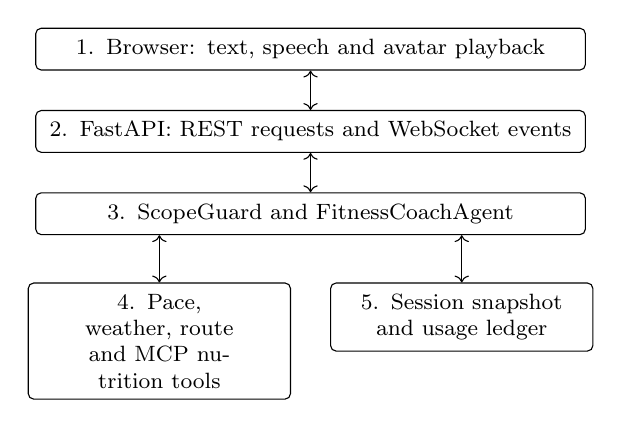
\begin{tikzpicture}[node distance=5mm]
\node[box,text width=6.7cm] (ui) {1. Browser: text, speech and avatar playback};
\node[box,below=of ui,text width=6.7cm] (api) {2. FastAPI: REST requests and WebSocket events};
\node[box,below=of api,text width=6.7cm] (agent) {3. ScopeGuard and FitnessCoachAgent};
\node[box,below=6mm of agent,xshift=-1.92cm,text width=3.05cm] (tools) {4. Pace, weather, route\\and MCP nutrition tools};
\node[box,below=6mm of agent,xshift=1.92cm,text width=3.05cm] (db) {5. Session snapshot\\and usage ledger};
\draw[<->] (ui)--(api);\draw[<->] (api)--(agent);
\draw[<->] (agent.south -| tools.north)--(tools.north);
\draw[<->] (agent.south -| db.north)--(db.north);
\end{tikzpicture}
\caption{The browser receives replies through the API. The agent accesses domain tools and persistent session state separately. MCP denotes Model Context Protocol.}\label{fig:arch}
\end{figure}

For a run with duration $t$ in minutes and distance $d>0$ in kilometres, pace is $p=t/d$ in minutes per kilometre. A 30-minute run over 5 km yields 6:00 min/km. Rounding is deferred until display. If the runner gives a number without a unit, the agent asks for the unit before saving the duration. A forecast additionally requires a place and time. Route length alone cannot resolve which forecast to use.

Figure~\ref{fig:flow} distinguishes requests that need clarification from requests ready for a tool. Algorithm~1 specifies a proposed accounting rule. Before a billable call, reserve an upper bound $r$ on its token cost. If actual usage is $u\leq r$, release $r-u$ tokens. With starting balance $B$, the resulting balance is $B-u$. A timeout with unknown usage keeps its reservation until reconciliation. Atomic reservations prevent two turns from spending the same balance.

\begin{figure}[htbp]\centering
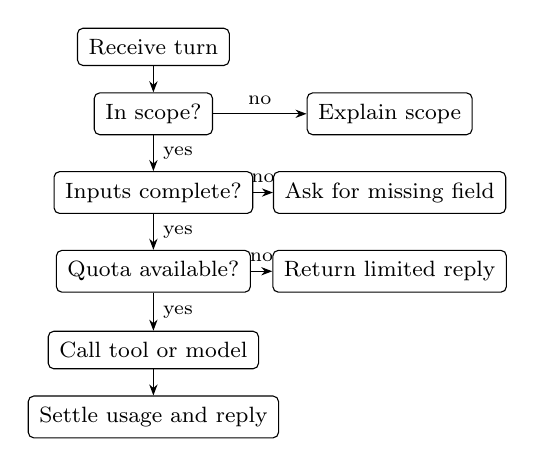
\begin{tikzpicture}
\node[box] (input) at (0,0) {Receive turn};
\node[box] (scope) at (0,-.85) {In scope?};
\node[box] (fields) at (0,-1.85) {Inputs complete?};
\node[box] (budget) at (0,-2.85) {Quota available?};
\node[box] (work) at (0,-3.85) {Call tool or model};
\node[box] (reply) at (0,-4.7) {Settle usage and reply};
\node[box] (redirect) at (3,-.85) {Explain scope};
\node[box] (ask) at (3,-1.85) {Ask for missing field};
\node[box] (stop) at (3,-2.85) {Return limited reply};
\draw[link] (input)--(scope);
\foreach \a/\b in {scope/fields,fields/budget,budget/work}{\draw[link] (\a)--node[right,font=\scriptsize]{yes}(\b);}
\foreach \a/\b in {scope/redirect,fields/ask,budget/stop}{\draw[link] (\a)--node[above,font=\scriptsize]{no}(\b);}
\draw[link] (work)--(reply);
\end{tikzpicture}
\caption{Decision path for one turn. Each right-hand branch returns control to the runner.}\label{fig:flow}
\end{figure}

\par\smallskip\noindent\textbf{Algorithm 1. Processing a coaching turn}\par
\begin{algorithmic}[1]
\STATE Load the snapshot and any completed reply for the turn ID.
\IF{the turn already has a completed reply}
  \STATE Return the stored reply.
\ENDIF
\STATE Apply ScopeGuard. Return guidance if outside scope.
\STATE Resolve units, place and time required by the intent.
\IF{a required field is missing}
  \STATE Save the pending intent, ask for the field and end turn.
\ENDIF
\FOR{each required call, up to the turn limit}
  \STATE Reserve its cost bound atomically or return a quota notice.
  \STATE Invoke the call and record the result or error.
  \STATE Settle known usage or flag the reservation for reconciliation.
  \IF{enough evidence is available, or a required call failed}
    \STATE Exit loop.
  \ENDIF
\ENDFOR
\STATE Save the evidence and reply under the turn ID.
\STATE Return text and, when requested and available, speech.
\end{algorithmic}

\subsection{Design tradeoffs}
The design preserves units, checks forecast validity, traces claims to tool outputs, reserves quota and retains confirmed inputs after reconnection. Three tradeoffs follow. Free-form requests can omit units, so the coach asks before calculating. A single agent shares context across tasks, so tools receive only the fields they need. Streaming can shorten the wait but can also speak an obsolete estimate, so numerical replies wait for the required evidence.

\subsection{Sensitivity of a run-before-rain decision}
Let $w$ be the number of minutes from departure to forecast rain onset, $d$ the route length in kilometres and $p$ the pace in minutes per kilometre. With no stops the time margin is $m=w-dp$. The break-even pace is $w/d$. For the 32-minute window in Table~\ref{tab:margin}, the 5~km break-even pace is 6:24 min/km. This number gives the runner a direct answer to a useful follow-up question: how fast would the loop have to be? At exactly that pace the runner reaches the finish at the forecast onset, with no time to spare.

Table~\ref{tab:grid} varies both route and pace while holding the window fixed. For a 4.5~km loop, even the slowest listed pace leaves 30~s. On the 5.5~km loop, even the fastest listed pace misses the window by one minute. Only the middle row changes sign. Asking about pace is therefore most consequential for that row. If the runner confirms 5.5~km and a pace in the stated range, the coach already has enough information to explain the shortfall and ask whether a shorter route is acceptable.

\begin{table}[tb]
\caption{Minutes until forecast onset after finishing. Calculated for a 32-minute window. Negative values mean finishing after onset.}
\label{tab:grid}\centering\small
\begin{tabular}{@{}lrrr@{}}\toprule
 & \multicolumn{3}{c}{Assumed pace (min/km)}\\
\cmidrule(l){2-4}
Route & 6:00 & 6:30 & 7:00\\\midrule
4.5 km & $+5.00$ & $+2.75$ & $+0.50$\\
5.0 km & $+2.00$ & $-0.50$ & $-3.00$\\
5.5 km & $-1.00$ & $-3.75$ & $-6.50$\\\bottomrule
\end{tabular}
\end{table}

The arithmetic also identifies when a yes-or-no answer overstates what is known. Suppose the weather tool reports an onset window from 17:29 to 17:35. A runner leaving at 17:00 for a 30-minute loop would finish one minute after the earliest onset or five minutes before the latest. Both outcomes fit the inputs. The reply can give the 17:30 finish and both margins. Assigning a probability to rain during the run would require an appropriate probability forecast. No frequency or forecast skill is inferred from the nine illustrative combinations in Table~\ref{tab:grid}.

\subsection{Corrections, interruptions and the cost of a retry}
A correction changes some derived values while leaving other facts intact. If the runner delays departure by ten minutes, the route distance and confirmed pace can be reused, but the earlier forecast must be checked against the revised outing. If the runner changes only a serving size, the referenced menu item can be retained. Given an illustrative entry of 180~kcal per 100~g, changing the portion from 150 to 100~g changes the saved estimate from 270 to 180~kcal. The proposed test reads the corrected record back and verifies both the quantity and the unit used for the calculation.

A lost connection presents a different ambiguity: the runner may not have heard the reply even though the service has completed a billable call. Consider a ledger with 1,000 tokens and two simultaneous requests that each need a reservation of 600. Under the proposed rule, one reservation leaves 400 available, which is insufficient for the other request. If the first call settles at 450, releasing the unused 150 leaves 550 available. Submitting that completed turn again should reproduce the stored reply and leave the balance at 550. The values are a worked test of the accounting rule. Measuring actual savings would require provider usage records and a defined comparison policy.

\section{Evaluation Protocol}
The original proposal describes a first-stage demonstration using a scripted account~\cite{proposal,project}. It connects an initial planning query to weather and route retrieval, adopting a plan, entering a run manually, correcting a food entry and retrieving the saved record. This is evidence that information can pass between functions. The proposal gives no attempt counts or turn-level logs from which to calculate a success rate, latency percentile or token saving. The protocol below specifies what to collect on the next run.
\subsection{Comparisons and measurement}
Run the same tasks through a form interface, the cloud agent and a local deployment of the same agent. For both agent deployments, fix the model, prompts, tool responses and token cap where possible. Test live services separately to expose network variation. Compare all three on field accuracy and task completion. Compare voice onset across voice-capable configurations. Report cold starts separately from warm turns, and retain failed turns in the completion denominator.

For the two shared tasks (computing pace and selecting a forecast for a revised departure), the minimum planned comparison is $2$ tasks $\times$ $3$ configurations $\times$ $30$ repetitions, or 180 attempts at one fixed load and start condition. Match inputs and rotate configuration order. Run voice and injected failures separately on applicable configurations. To isolate avatar overhead, repeat the same voice request with lip synchronization enabled and disabled. Scripted repetitions measure service behavior under the chosen conditions. Estimating time saved by runners would require observing runners using the interfaces.

Table~\ref{tab:metrics} defines the four timing endpoints in the project proposal~\cite{proposal}. Within each condition, sort the $n$ successful timed trials and take rank $\lceil0.95n\rceil$ for P95. With 30 successes, P95 is the second-slowest time. If only 24 of 30 attempts succeed, the latency summary covers those 24 and completion is 80\%. If none succeeds, P95 is undefined. Publish the denominators beside the timings. Vary the token cap and concurrency to identify where either completion or latency deteriorates.

\begin{table}[tb]
\caption{Proposed response targets. Clocks start and stop at the client. The first three targets apply to P95.}
\label{tab:metrics}\centering\footnotesize
\begin{tabularx}{\columnwidth}{@{}lYr@{}}\toprule
Interaction & Timing interval & Target\\\midrule
Page query & Submit to visible data & $<2$~s\\
Text reply & Submit to first text that addresses the task & $<8$~s\\
Voice reply & End of speech to first audible reply & $<12$~s\\
Interrupt & Stop command to playback silence & $<300$~ms\\\bottomrule
\end{tabularx}
\end{table}

Score each attempted task against the expected outcome below. For valid pace inputs, report absolute error in seconds per kilometre against $60t/d$ and count missing replies separately. For forecast tasks, check both the location and the validity interval. Record clarification turns per attempt. Divide all billed tokens, including those spent on failed attempts, by the number of completed tasks. For factual replies, report the fraction whose material claims all trace to valid tool results or confirmed inputs. Here a completed task is one meeting the expected outcome. When none completes, the token ratio is undefined. These measures expose cases in which a quick reply is incomplete or a low token count reflects an early failure.
\subsection{Ten questions for validating the coach}
Each question has an observable answer for a scripted test.
\begin{enumerate}
\item What pace follows from 5 km in 30 min? The expected value is 6:00 min/km.
\item How is zero distance handled? The client requests a positive distance and displays no pace.
\item What happens when units are omitted? The next turn asks for the unit and preserves the number.
\item Which forecast fits a changed departure time? Its validity interval must cover the updated time at the requested location.
\item What if a route lookup times out? The reply identifies the missing route and omits its length.
\item Where did a meal estimate come from? The trace links it to an MCP result and its portion size.
\item Does an unrelated request use a domain tool? The trace ends at ScopeGuard before such a call runs.
\item Can concurrent turns exceed the balance? Settled usage plus active reservations must stay within the starting quota.
\item Does reconnecting duplicate a completed turn? Resubmitting its ID returns the stored reply and leaves the ledger unchanged.
\item When does the avatar respond? Record the offset between first audible speech and first mouth motion separately from voice onset.
\end{enumerate}
Unit tests check arithmetic and quota updates. Integration tests inject stale forecasts, timeouts and duplicate IDs. A browser smoke test covers spoken input through playback.

\subsection{Reading the results of the planned comparison}
The primary unit of analysis is a complete request from its first input through the expected final answer or saved state. A clarification is part of that same attempt. For example, if the speaker omits a unit, a correct clarifying question earns credit for identifying the omission. The task counts as complete only after the scripted user supplies the unit and the service gives the expected calculation. This avoids favoring an interface that quickly asks a question and never finishes the job.

Use the same route record and forecast fixture for all three interfaces in a matched comparison. For a changed departure, prepare one case where the revised time stays inside the forecast interval and one where it falls outside. In the first, reusing the forecast is appropriate. In the second, the reply needs an updated observation or an explicit statement that the forecast is unavailable. Score the task with its expected outcome before looking at response times. Testing live forecasts separately then reveals service delay without changing the answer key mid-comparison.

Report a deadline measure alongside successful-turn latency. Its numerator is the number of attempts that both reached the correct outcome and did so before the relevant deadline. Its denominator is all eligible attempts in that condition, including timeouts and quota refusals. For example, if 24 of 30 attempts finish correctly and 22 of those finish before the deadline, completion is 80.0\% and on-time completion is 73.3\%. A fast acknowledgement alone satisfies neither condition. These illustrative counts explain how a favorable P95 among successes could coexist with a poor experience for some runners.

The initial 30 repetitions per condition provide coarse information about rare delays: one outcome changes a reported rate by 3.3 percentage points. Report the numerator and denominator for each task before aggregating. Keep cold-start requests, live-service interruptions and errors in the answer itself distinguishable in the trace. A long voice delay with prompt text already available points to a different part of the system than a reply delayed while waiting for a route lookup. This separation makes it possible to prioritize the next engineering change once actual traces exist.

\section{Conclusion}
The demonstration linked a runner's question to tools and a spoken reply. The proposed comparison will show when that reply arrives in time, when it is correct and how often quota limits interrupt the task. GPS, step counts and posture sensing remain future work and require separate validation.

\begin{thebibliography}{00}
\bibitem{strava} Strava, \emph{12th Annual Year in Sport Trend Report}, Dec. 3, 2025. \href{https://press.strava.com/en-gb/articles/strava-releases-12th-annual-year-in-sport-trend-report-2025}{Online report}.
\bibitem{proposal} \emph{AI Fitness Coach: A Conversational Running Coach}, original course proposal, Nov. 10, 2026, in Chinese, pp. 1--4. \href{https://github.com/HitomiHuang/DIC3-AI-Fitness-Coach/blob/main/myplan/proposal.pdf}{Project proposal}.
\bibitem{project} \emph{AI Fitness Coach Proposal Analysis}, course project review, pp. 1--2, undated, in Chinese. Supplied with the project infographic.
\bibitem{react} S. Yao \emph{et al.}, \textquotedblleft ReAct: Synergizing reasoning and acting in language models,\textquotedblright\ in \emph{Proc. Int. Conf. Learning Representations}, 2023. \href{https://react-lm.github.io/}{Project and paper}.
\bibitem{phllm} J. Khasentino \emph{et al.}, \textquotedblleft A personal health large language model for sleep and fitness coaching,\textquotedblright\ \emph{Nature Medicine}, vol. 31, pp. 3394--3403, 2025, \href{https://doi.org/10.1038/s41591-025-03888-0}{doi: 10.1038/s41591-025-03888-0}.
\bibitem{heat} N. El Helou \emph{et al.}, \textquotedblleft Impact of environmental parameters on marathon running performance,\textquotedblright\ \emph{PLOS ONE}, vol. 7, no. 5, Art. no. e37407, 2012, \href{https://doi.org/10.1371/journal.pone.0037407}{doi: 10.1371/journal.pone.0037407}.
\bibitem{tau} S. Yao, N. Shinn, P. Razavi, and K. Narasimhan, \textquotedblleft $\tau$-bench: A benchmark for tool-agent-user interaction in real-world domains,\textquotedblright\ \emph{arXiv:2406.12045}, 2024. \href{https://arxiv.org/abs/2406.12045}{Paper}.
\bibitem{gnss} R. Gilgen-Ammann, T. Schweizer, and T. Wyss, \textquotedblleft Accuracy of distance recordings in eight positioning-enabled sport watches: Instrument validation study,\textquotedblright\ \emph{JMIR mHealth and uHealth}, vol. 8, no. 6, e17118, 2020. \href{https://doi.org/10.2196/17118}{doi: 10.2196/17118}.
\bibitem{nutri} Q. Thames \emph{et al.}, \textquotedblleft Nutrition5k: Towards automatic nutritional understanding of generic food,\textquotedblright\ in \emph{Proc. IEEE/CVF Conf. Computer Vision and Pattern Recognition}, 2021, pp. 8903--8911. \href{https://openaccess.thecvf.com/content/CVPR2021/html/Thames_Nutrition5k_Towards_Automatic_Nutritional_Understanding_of_Generic_Food_CVPR_2021_paper.html}{Paper}.

\end{thebibliography}
\end{document}
